\documentclass[a4paper,12pt]{article}
\usepackage{setspace}
\usepackage{indentfirst}
\usepackage{graphicx}
\usepackage[UTF8]{ctex}
\usepackage{amsmath} 
\usepackage[dvipsnames]{xcolor}
\usepackage{listings}
\usepackage{indentfirst}
\usepackage{xcolor}
\lstset { %
    language=C++,
    backgroundcolor=\color{black!5}, % set backgroundcolor
    basicstyle=\footnotesize,% basic font setting
}
\begin{document}
\title{C++ 学习笔记}
\date{\today}
\maketitle
\begin{spacing}{2}
\pagenumbering{arabic}
\tableofcontents
\newpage
\pagenumbering{arabic}
\end{spacing}
\begin{spacing}{2}
\section{指针,数组,结构体}
\subsubsection{在输入字符的时候有三种情况}:
\begin{itemize}
\item 当输入两次字符串并且需要换行的时候,可以用cin.getline()或者cin.get()两种方法代替
\begin{lstlisting}
cout<<"Enter your name:";
cin>>name;
cout<<"Enter name of dessert:";
cin>>dessert;
\end{lstlisting}
假如是以上情况,那么未能等到输入dessert的名字的时候,就结束了。这是因为cin通过使用空白(空格,制表符和换行符)来确定字符串的结束位置,这意
味着cin在获取字符数组输入时只读取一个字符。
\item 所以可以使用cin.getline(变量名,数组长度)。或者cin.get(变量名,数组长度)。但在使用cin.get()也需要注意的是,当使用第一次cin.get()之后,在第一次调用换行符还在输入列中,因此第二次调用cin.get()的时候看到的第一个字符便是换行符,因此get()认为已经到了结尾,而没发现任何可以读取的内容。
\begin{lstlisting}
cin.get(name,size);
cin.get();
cin.get(dessert,size);
\end{lstlisting}
\item 在输入数字之后,由于回车键生成的换行符留在了输入列中,cin.getline()看到换行符之后,将认为是一个空行,想继续输入字符的话,可以调用cin.get()方法
\begin{lstlisting}
int year;
cin>>year;
cin.get(name,size);

(cin>>year).get();
cin.getline(name,size);
\end{lstlisting}
\end{itemize}
同时,要始终记住cin以空格,制表符,换行符为结束标志,所以输入字符串到某一个点结束可以用如下代码
\begin{lstlisting}
#include <iostream>  
#include <string>  
using namespace std;
int main()
{
    cout << "Enter words (to stop, type the word done):" << endl;
    string str;
    int count = 0;
    while (cin >> str && str != "done")
        count++;
    cout << count << endl;

    system("pause");
    return 0;
}
\end{lstlisting}
\subsubsection{自动存储、静态存和动态存储}
\begin{itemize}
\item\textbf{自动存储}当函数内部定义的常规变量使用自动存储空间,被称为自动变量,这意味着它们在所属的函数被调用时自动产生,在该函数结束时消亡。自动变量通常存储在\textbf{栈}中。这意味着执行代码块时,其中的变量将依次加入到栈中,而在离开代码块时,将按照相反的顺序释放这些变量,这被称为后进先出。因此,在程序执行过程中,栈将不断放大缩小
\item\textbf{静态存储}静态存储是整个程序执行期间都存在的存储方式。使变量成为静态的方式有两种:一种是在函数外面;另一种实在变量时使用关键词:static:
\begin{lstlisting}
double increase()
{
	static double fee = 56.5;
	fee = fee + 1;
	return fee;
		
}
int main()

{
	double  a=increase();
	cout << a << endl;
	float b=increase();
	cout << b;
	return 0;

}
\end{lstlisting}a=57.5,b=58.5因为在每一次调用fee本身都会增加一,并不会随着increase()结束调用而消亡。
\item \textbf{动态存储} new 和delete 运算符提供了一种比自动变量和静态变量更灵活的方法。它们管理了一个内存池吗,在C++中被称为自由存储空间(free store)或 堆(heap)。该内存池用于静态变量和自动变量的内存是分开的。
\item \textbf{**的用法}
\begin{lstlisting}
#include<iostream>
#include <stdio.h>
#include<string>
#include<cctype>
using namespace std;
struct antarctica_years_end
{
	int year;
};
int main()

{
	antarctica_years_end  s01, s02, s03;
	s01.year = 1998;
	antarctica_years_end* pa = &s02;
	pa->year = 1999;
	antarctica_years_end trio[3];
	trio[0].year = 2003;
	cout << trio->year << endl;
	const  antarctica_years_end* arp[3] = { &s01,&s02,&s03 };
	cout << arp[1]->year << endl;
	const antarctica_years_end** ppa = arp;
	auto ppb = arp;
	cout << (*ppb)->year << endl;
	cout << (*(ppb+1))->year << endl;
	return 0;

}
\end{lstlisting}
\begin{figure}[h]
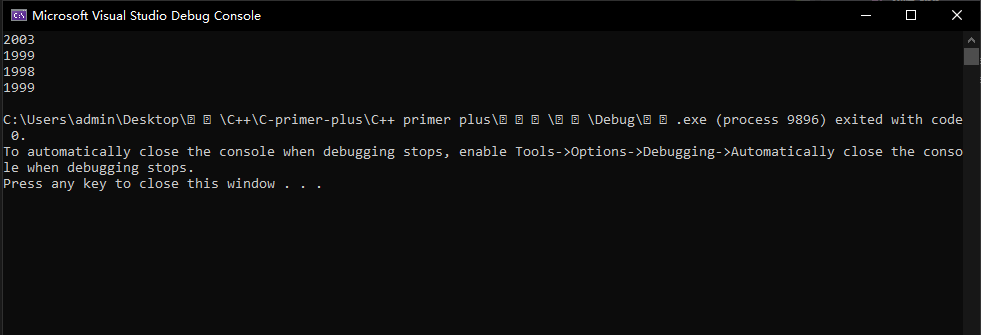
\includegraphics[scale=1]{Figure 1.PNG}
\caption{**基本输出}
\label{figure 1}
\end{figure}
\end{itemize}
\section{循环和关系表达式}
遍历一个字符串,可以通过while loop:
\begin{lstlisting}
int i=0;
while (name[0]!='\0')
{
  cout<<name[i]<<":"<<int(name[i])<<endl;
  i++;
}
return 0;
\end{lstlisting}
\paragraph{ }指针的方式
\begin{lstlisting}
#include<iostream>
using namespace std;
int main()
{
    const char* name = "sadas";
	cout << name << endl;
	
	while (*name)
	{
		cout << *name << endl;
		name++;
	}
	return 0;
}
\end{lstlisting}
int(name[i])可以将ASCII 码转换成对应的数字
\paragraph{}无限循环的两中方式:
\begin{itemize}
\item for(;;)
\item while true
\end{itemize}
\paragraph{ }编写延时循环
\begin{lstlisting}
long wait=0;
while(wait<10000)
   wait++;
\end{lstlisting}
这种方法的问题是,当计算机处理器的速度发生变化时,必须修改计数限制。
可以使用ctime库函数。
\begin{lstlisting}
#include<iostream>
#include<ctime>
using namespace std;
int main()
{
	cout << "Enter the delay time in seconds:";
	float secs;
	cin >> secs;
	clock_t delay = secs * CLOCKS_PER_SEC;
	cout << "Starting\a\n";
	clock_t start = clock();
	while (clock() - start < delay)
		;
	cout << "done\a\n";
	return 0;
}
\end{lstlisting}
\subsection{C++为类型建立别名的方式有两种}
\begin{itemize}
\item $\#$define BYTE char
\item typedef char byte(typedef typeName aliasName)
\end{itemize}
\subsection{基于范围的for循环}
\paragraph{ }打印一个数组所有的元素
\begin{lstlisting}
    double prices[5] = { 1.2,2.3,4.1,3.2,1.6 };
	for (double x : prices)
	{
		cout << x << endl;

	}
	return 0;
\end{lstlisting}
\subsubsection{要修改数组的元素}
\begin{lstlisting}
    double prices[5] = { 1.2,2.3,4.1,3.2,1.6 };
	for (double &x : prices)
	{
		x = x * 0.8;
		cout << x << endl;

	}
	return 0;
\end{lstlisting}
或者基于范围的for循环和初始化列表:
\begin{lstlisting}
    for(int x:{3,5,2,8,6})
       cout<<x;
\end{lstlisting}
\begin{center}
\begin{table}[ht]
\caption{cin.get(ch)与 cin.get()} % title of Table
\centering % used for centering table
\begin{tabular}{c|c|c  } % centered columns (3 columns)
\hline\hline %inserts double horizontal lines
属性 &cin.get(ch) &ch==cin.get() \\ [0.5ex] % inserts table
%heading
\hline % inserts single horizontal line
 传递输入字符的方式& 赋给参数ch & 将函数返回赋值给ch  \\
 \hline
用于字符输入时函数的返回值 & istream对象(执行bool转换后为true) & int 类型的字符编码  \\
\hline
到达EOF时函数的返回值& istream对象(执行bool转换之后为false) &EOF  \\
\hline %inserts single line
\end{tabular}
\label{table:nonlin} % is used to refer this table in the text
\end{table}
\end{center}
\section{const 和指针的使用}
\begin{lstlisting}
int a=30;
const int *ps=&a;
int *const finger=&a;
\end{lstlisting}
上述情况中,const关键字位置不同。这使得finger 只能指向a的位置,但是可以通过修改*finger的值来修改a的值,而ps可以重新指向另一个变量的位置,但是不能修改自己本身*ps的值。
另一种情况,还可以声明指向const对象的const指针。
\begin{lstlisting}
double trouble=2.3E30;
const double*const stick=&trouble;
\end{lstlisting}
其中stick只能指向trouble,且stick不可修改trouble的值,简而言之strick和*stcick都是const。 
\end{spacing}
\end{document}